\documentclass[12pt]{article}
\usepackage[a4paper, total={6in, 9in}]{geometry}
\usepackage{graphicx}
\graphicspath{ {./images/output/} }
\usepackage{caption}
\usepackage[english]{babel}
\usepackage{titling}
\usepackage{float}
\usepackage{amsmath}
\usepackage{minted}
\usepackage{multicol}
% \usepackage{array}
% \usepackage{setspace}
% \usepackage{placeins}
\setlength{\parindent}{0pt}

% \usepackage{lipsum}

\title{Study of Amplitude \& DSB\-SC-SC Modulation \& Demodulation}
\author{}
\date{}

\pagenumbering{gobble}
\begin{document}
\vspace*{\fill}
\begin{center}

    \emph{Heaven's Light is Our Guide} \\
    \textbf{Rajshahi University of Engineering and Technology} \\

    \begin{figure}[H]
        \centering
        
\includegraphics[scale=.34]{images/RUET_logo.png}
        \label{fig:ruet_logo}
    \end{figure}
    \vspace{5mm}

    \textbf{Course Code}\\
    ECE 3208\\
    \vspace{3mm}
    \textbf{Course Title}\\
    Communication Engineering Sessional

    \vspace{5mm}
    \textbf{Experiment Date:} {January 21, 2025},\\
    \textbf{Submission Date:} {February 11, 2025}\\

    \vspace{5mm}
    \textbf{Lab Report 3: \\
        Determination of Modulation Index of FM Wave}

    \vspace{15mm}

    \begin{tabular}{c|c}
        \textbf{Submitted to} & \textbf{Submitted by} \\
        Dr. Md. Kamal Hosain  & Md. Tajim An Noor     \\
        Professor             & Roll: 2010025         \\
        Dept of ETE, RUET     &                       \\
    \end{tabular}

\end{center}
\vspace*{\fill}


\pagebreak

\tableofcontents

\pagebreak
\pagenumbering{arabic}
\maketitle

\section*{Theory}
\addcontentsline{toc}{section}{Theory}
Amplitude Modulation (AM) is a modulation technique used in electronic communication, most commonly for transmitting information via a radio carrier wave. In AM, the amplitude of the carrier signal is varied in proportion to that of the message signal, such as an audio signal. This technique is used in a variety of applications, including broadcasting and two-way radio communication \cite{haykin2008communication}.
\\\\
Double Sideband Suppressed Carrier (DSB\-SC-SC) is a type of amplitude modulation that suppresses the carrier frequency, leaving only the upper and lower sidebands. This results in a more power-efficient transmission since the carrier does not need to be transmitted. DSB\-SC-SC is used in applications where bandwidth efficiency is crucial, such as in certain types of radio communication systems \cite{proakis2007digital}.
\\\\
In this experiment, we will study the principles of AM and DSB\-SC-SC modulation and demodulation. We will generate AM and DSB\-SC-SC signals, observe their spectra, and demodulate them to recover the original message signal. The experiment will help us understand the advantages and disadvantages of each modulation technique and their practical applications.

\subsection*{AM Modulation}
AM modulation involves varying the amplitude of a high-frequency carrier signal in accordance with the instantaneous amplitude of the message signal. The mathematical representation of an AM signal is given by:
\[
    s(t) = [A + m(t)] \cos(2 \pi f_c t)
\]
where \(A\) is the carrier amplitude, \(m(t)\) is the message signal, and \(f_c\) is the carrier frequency.

\begin{figure}[H]
    \centering
    % \includegraphics[width=0.8\textwidth]{am_modulation.png}
    \caption{AM Modulation}
    \label{fig:am_modulation}
\end{figure}

\subsection*{DSB\-SC-SC Modulation}
DSB\-SC-SC modulation is achieved by multiplying the message signal with the carrier signal. The mathematical representation of a DSB\-SC-SC signal is:
\[
    s(t) = m(t) \cos(2 \pi f_c t)
\]
This results in a signal that contains only the sidebands, with the carrier suppressed.

\begin{figure}[H]
    \centering
    % \includegraphics[width=0.8\textwidth]{dsb_sc_modulation.png}
    \caption{DSB\-SC-SC Modulation}
    \label{fig:dsb_sc_modulation}
\end{figure}

\subsection*{Demodulation}
Demodulation is the process of extracting the original message signal from the modulated carrier. For AM signals, this can be achieved using an envelope detector. For DSB\-SC-SC signals, coherent detection is required, which involves mixing the received signal with a locally generated carrier signal that is synchronized in frequency and phase with the original carrier.

\section*{Required Apparatus}
\addcontentsline{toc}{section}{Required Apparatus}
\begin{itemize}
    \item ANALOGUE SIGNAL PROCESSING DL 3155M60R
    \item Oscilloscope
    \item Connecting Wires
\end{itemize}

\section*{Block Diagram}
\addcontentsline{toc}{section}{Block Diagram}
\subsection*{AM and DSB\-SC-SC Modulation Block Diagram}
\begin{figure}[H]
    \centering
    % \includegraphics[width=0.8\textwidth]{modulation_block_diagram.png}
    \caption{Block Diagram of AM and DSB\-SC-SC Modulation}
    \label{fig:modulation_block_diagram}
\end{figure}

\subsection*{AM and DSB\-SC-SC Modulation and Demodulation Block Diagram}
\begin{figure}[H]
    \centering
    % \includegraphics[width=0.8\textwidth]{modulation_demodulation_block_diagram.png}
    \caption{Block Diagram of AM and DSB\-SC-SC Modulation and Demodulation}
    \label{fig:modulation_demodulation_block_diagram}
\end{figure}

\section*{Procedure}
\addcontentsline{toc}{section}{Procedure}
\begin{enumerate}
    \item A function generator was used to generate two signals: a lower frequency message signal and a higher frequency carrier signal.
    \item The AM/SSB/DSBSC board (ACT-02 AM DSB\-SC-SC/SSB Kit) was used, specifically the balanced modulator portion of the board for the first experiment.
    \item The message signal was passed to the balanced modulator, and the waveshapes of the message, carrier, and modulated signals were observed.
    \item By adjusting the knob, AM and DSB\-SC-SC modulation were performed. Under, over, and 100\% modulation were observed for AM modulation. For DSB\-SC-SC, the message amplitude was varied to observe cases similar to AM under or over modulation.
    \item Another balanced modulator was used to pass the modulated signal through, and the output was then passed through a low pass filter to recover the original message signal for both AM and DSB\-SC-SC.
    \item The waveforms were observed on the oscilloscope at each step.
\end{enumerate}

\section*{Experimental Data}
\addcontentsline{toc}{section}{Experimental Data}
\begin{table}[H]
    \centering
    \begin{tabular}{|c|c|c|c|c|c|c|}
        \hline
        \textbf{Modulation Type} & \textbf{A\textsubscript{m}} & \textbf{F\textsubscript{m}} & \textbf{A\textsubscript{c}} & \textbf{F\textsubscript{c}} & \textbf{A\textsubscript{max}} & \textbf{A\textsubscript{min}} \\
        \hline
        AM Under Modulation      & 0.4V                        & 1.75kHz                     & 2.2V                        & 298.8kHz                    & 2.52V                         & 0.5V                          \\
        \hline
        AM 100\% Modulation      & 0.54V                       & 1.762kHz                    & 2.22V                       & 301.5kHz                    & 2.54V                         & 0V                            \\
        \hline
        AM Over Modulation       & 0.9V                        & 1.75kHz                     & 2.24V                       & 300.32kHz                   & 2.64V                         & 1.2V                          \\
        \hline
        DSB-SC Modulation 1      & 0.9V                        & 1.75kHz                     & 2.28V                       & 300.3kHz                    & -                             & -                             \\
        \hline
        DSB-SC Modulation 1      & 1.88V                       & 1.75kHz                     & 2.28V                       & 300.3kHz                    & -                             & -                             \\
        \hline
    \end{tabular}
    \caption{Experimental Data for Modulation Types}
    \label{tab:experimental_data}
\end{table}

\section*{Calculations}
\addcontentsline{toc}{section}{Calculations}
The modulation index (\( \mu \)) for AM can be calculated using the formula:
\[
    \mu = \frac{A_{\text{max}} - A_{\text{min}}}{A_{\text{max}} + A_{\text{min}}}
\]

\subsection*{AM Under Modulation}
Given:
\[
    A_{\text{max}} = 2.52V, \quad A_{\text{min}} = 0.5V
\]
\[
    \mu = \frac{2.52 - 0.5}{2.52 + 0.5} = \frac{2.02}{3.02} \approx 0.668
\]

\subsection*{AM 100\% Modulation}
Given:
\[
    A_{\text{max}} = 2.54V, \quad A_{\text{min}} = 0V
\]
\[
    \mu = \frac{2.54 - 0}{2.54 + 0} = \frac{2.54}{2.54} = 1
\]

\subsection*{AM Over Modulation}
Given:
\[
    A_{\text{max}} = 2.64V, \quad A_{\text{min}} = 1.2V
\]
\[
    \mu = \frac{2.64 - (-1.2)}{2.64 + (-1.2)} = \frac{3.84}{1.44} \approx 2.67
\]

For DSB-SC modulation, the modulation index is not applicable as the carrier is suppressed.

\section*{Matlab Simulation}
\addcontentsline{toc}{section}{Matlab Simulation}

\subsection*{Code (AM):}
\addcontentsline{toc}{subsection}{Code (AM)}
The following Matlab code simulates the generation, modulation, and demodulation of an analog signal using Amplitude Modulation (AM).

\inputminted[linenos,breaklines,breakanywhere]{matlab}{./assets/am.m}

\subsection*{Code (DSB\-SC-SC):}
\addcontentsline{toc}{subsection}{Code (DSB\-SC-SC)}
The following Matlab code simulates the generation, modulation, and demodulation of an analog signal using Double Sideband Suppressed Carrier (DSB\-SC-SC) modulation.

\inputminted[linenos,breaklines,breakanywhere]{matlab}{./assets/dsb-sc.m}

\section*{Output}
\addcontentsline{toc}{section}{Output}

\subsection*{Experimental Output}
\addcontentsline{toc}{subsection}{Experimental Output}
\begin{figure}[H]
    \centering
    \begin{minipage}{0.45\linewidth}
        \centering
        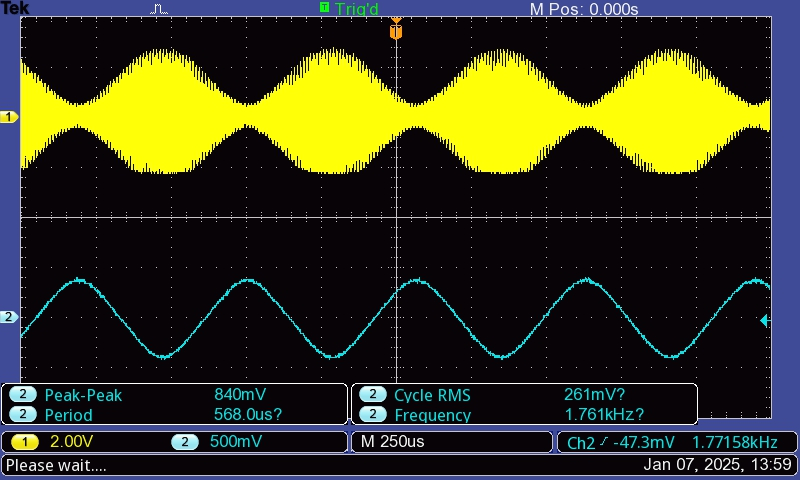
\includegraphics[width=\linewidth]{p1-undMod-msg.JPG}
        \caption{AM; Yellow: Under-modulated, Blue: Message}
        \label{fig:pic1}
    \end{minipage}
    \hfill
    \begin{minipage}{0.45\linewidth}
        \centering
        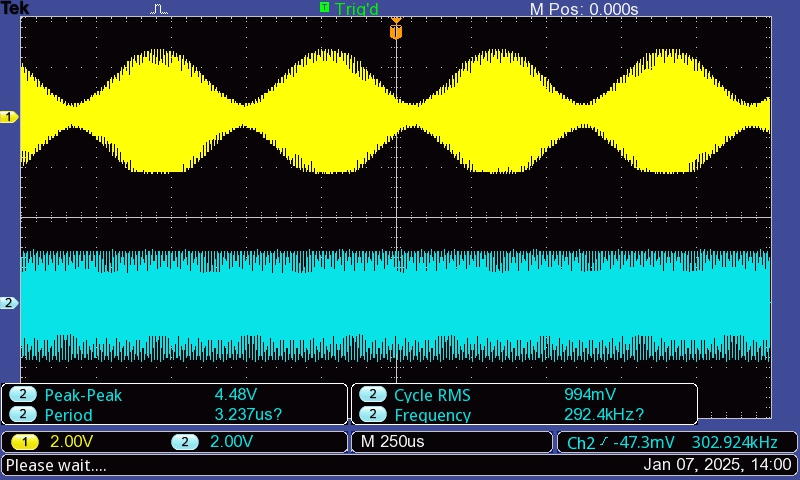
\includegraphics[width=\linewidth]{p2-undMod-car.JPG}
        \caption{AM; Yellow: Under-modulated, Blue: Carrier}
        \label{fig:pic2}
    \end{minipage}
    \vspace{1em}
    \begin{minipage}{0.45\linewidth}
        \centering
        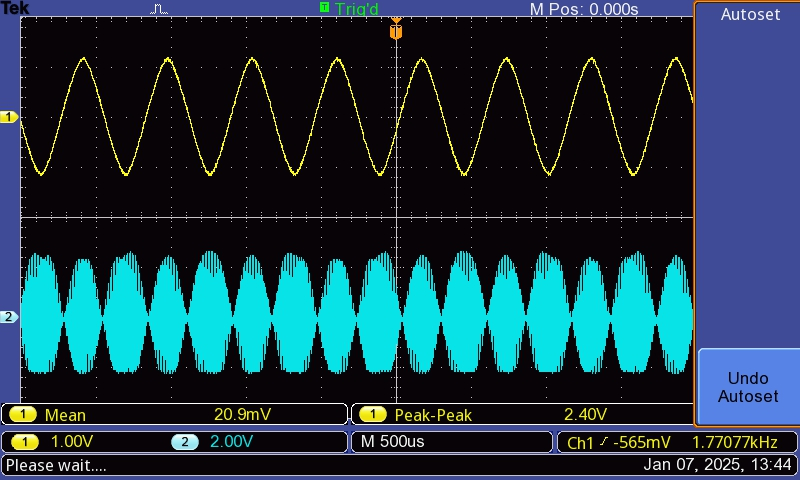
\includegraphics[width=\linewidth]{p3-msg-100mod.JPG}
        \caption{AM; Yellow: Message, Blue: 100\% Modulated}
        \label{fig:pic3}
    \end{minipage}
    \hfill
    \begin{minipage}{0.45\linewidth}
        \centering
        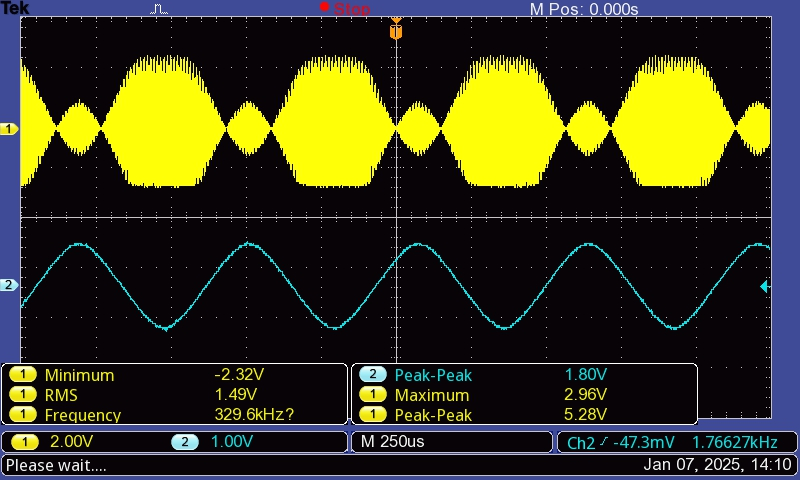
\includegraphics[width=\linewidth]{p4-ovMod-msg.JPG}
        \caption{AM; Yellow: Over-modulated, Blue: Message}
        \label{fig:pic4}
    \end{minipage}
    \vspace{1em}
    \begin{minipage}{0.45\linewidth}
        \centering
        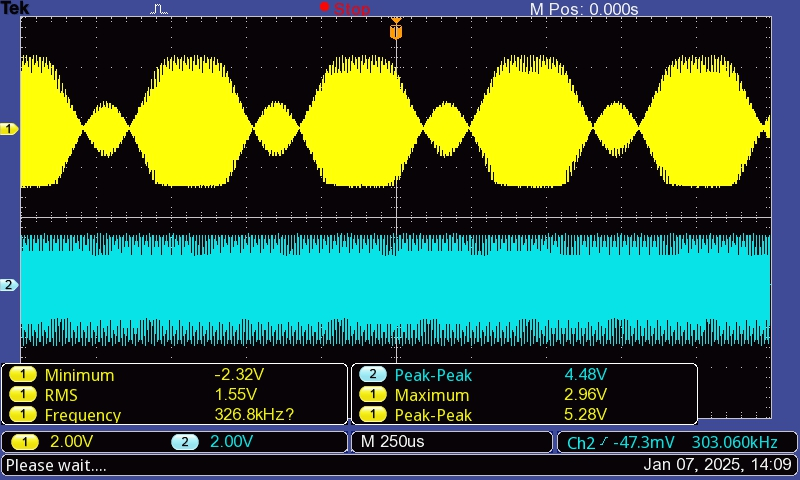
\includegraphics[width=\linewidth]{p5-ovMod-car.JPG}
        \caption{AM; Yellow: Over-modulated, Blue: Carrier}
        \label{fig:pic5}
    \end{minipage}
    \hfill
    \begin{minipage}{0.45\linewidth}
        \centering
        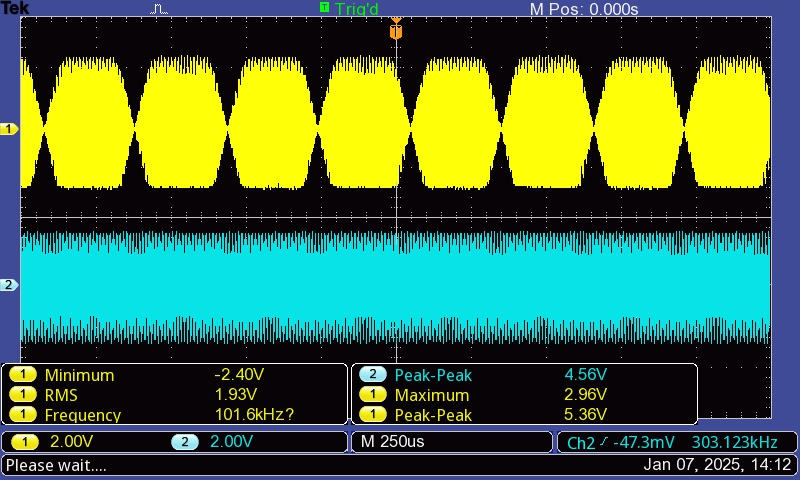
\includegraphics[width=\linewidth]{p6-dsb-mod-car.JPG}
        \caption{DSB\-SC; Yellow: Modulated, Blue: Carrier}
        \label{fig:pic6}
    \end{minipage}
\end{figure}

\pagebreak

\begin{figure}[H]
    \centering
    \begin{minipage}{0.45\linewidth}
        \centering
        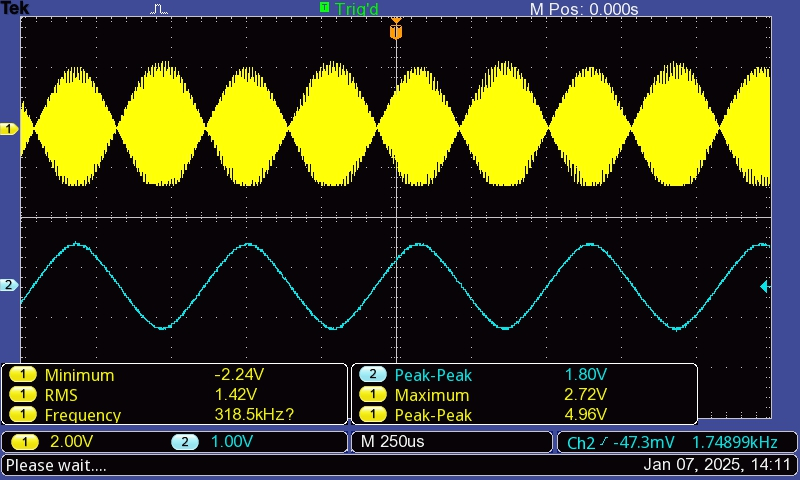
\includegraphics[width=\linewidth]{p7-dsb-mod-msg.JPG}
        \caption{DSB\-SC; Yellow: Modulated, Blue: Message 1}
        \label{fig:pic7}
    \end{minipage}
    \hfill
    \begin{minipage}{0.45\linewidth}
        \centering
        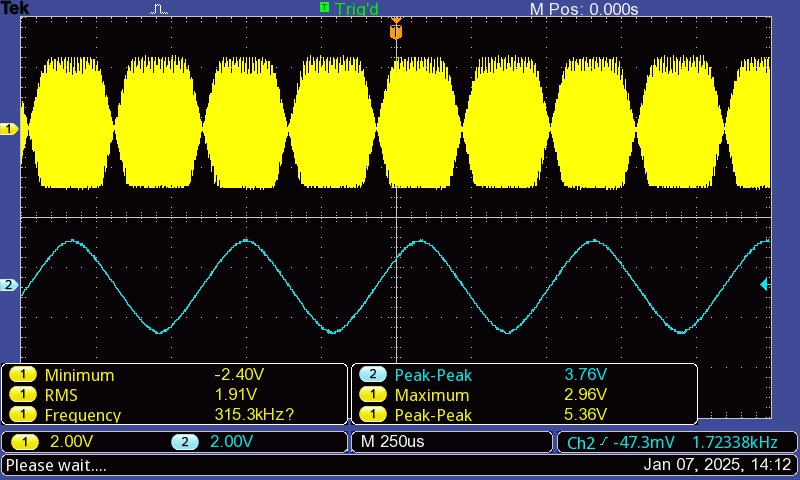
\includegraphics[width=\linewidth]{p8-dsb-mod-msg2.JPG}
        \caption{DSB\-SC; Yellow: Modulated, Blue: Message 2}
        \label{fig:pic8}
    \end{minipage}
    \vspace{1em}
    \begin{minipage}{\linewidth}
        \centering
        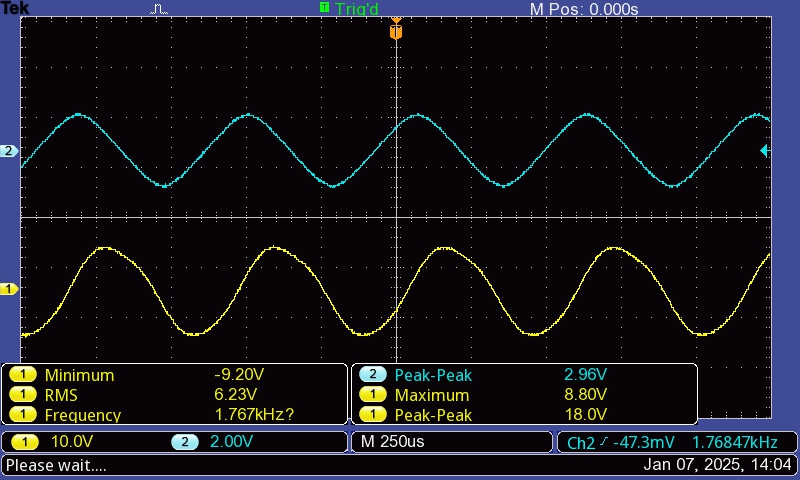
\includegraphics[width=0.4\linewidth]{p9-dsb-msg-Demod.JPG}
        \caption{DSB\-SC; Yellow: Message, Blue: Demodulated Message}
        \label{fig:pic9}
    \end{minipage}
\end{figure}

\subsection*{Matlab Simulation Output}
\addcontentsline{toc}{subsection}{Matlab Output}
\begin{figure}[H]
    \centering
    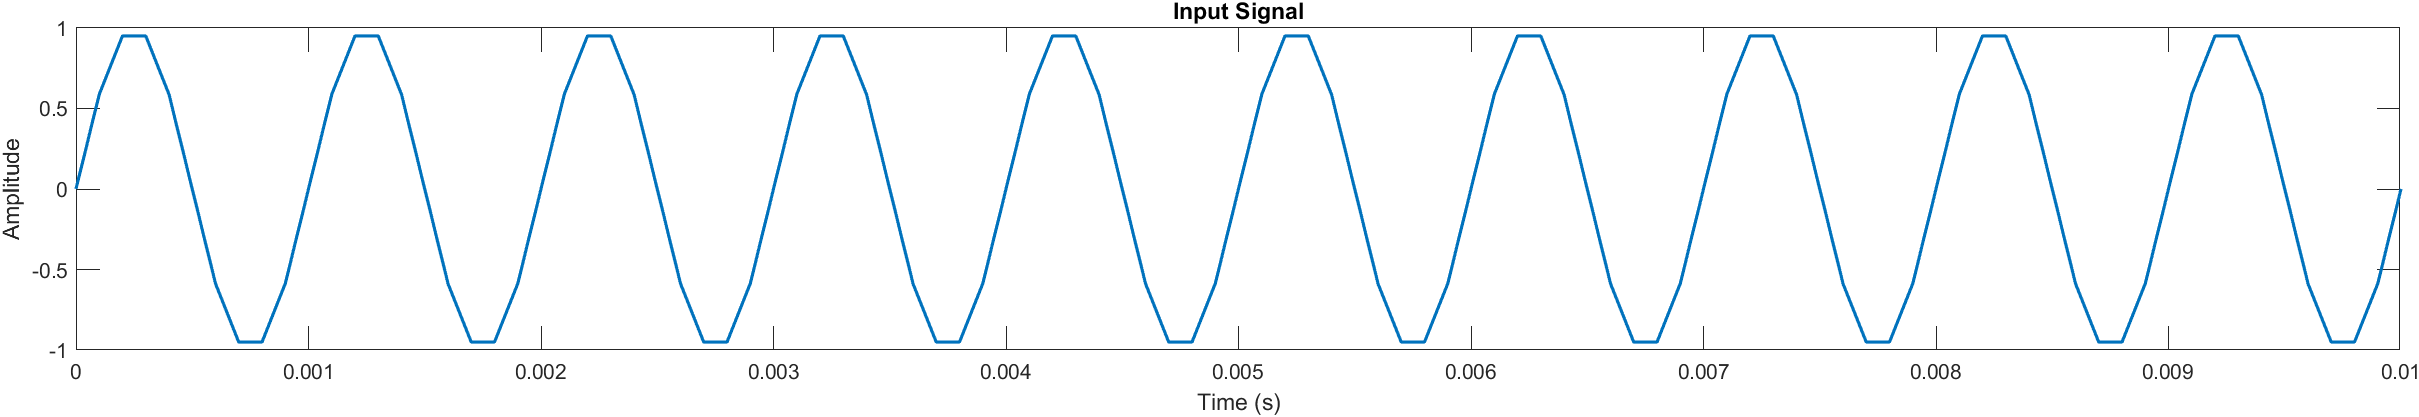
\includegraphics[width=\textwidth]{msg.png}
    \caption{Message Signal}
    \label{fig:img2}
\end{figure}

\begin{figure}[H]
    \centering
    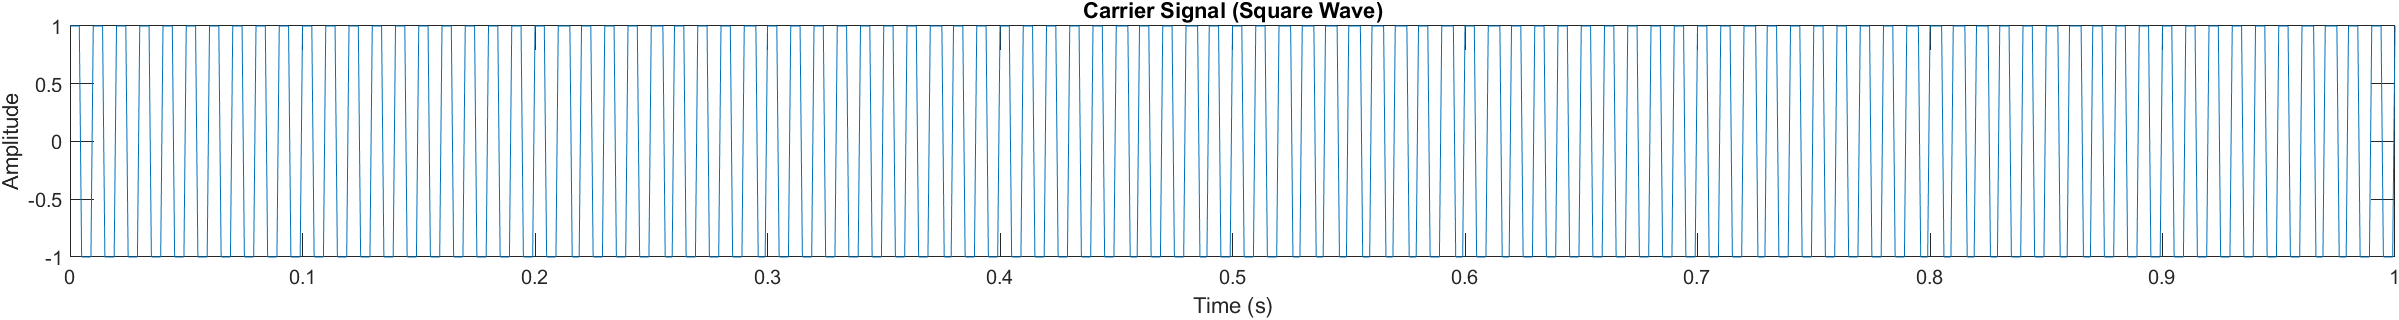
\includegraphics[width=\textwidth]{car.png}
    \caption{Carrier Signal, Square Wave}
    \label{fig:img11}
\end{figure}

\begin{figure}[H]
    \centering
    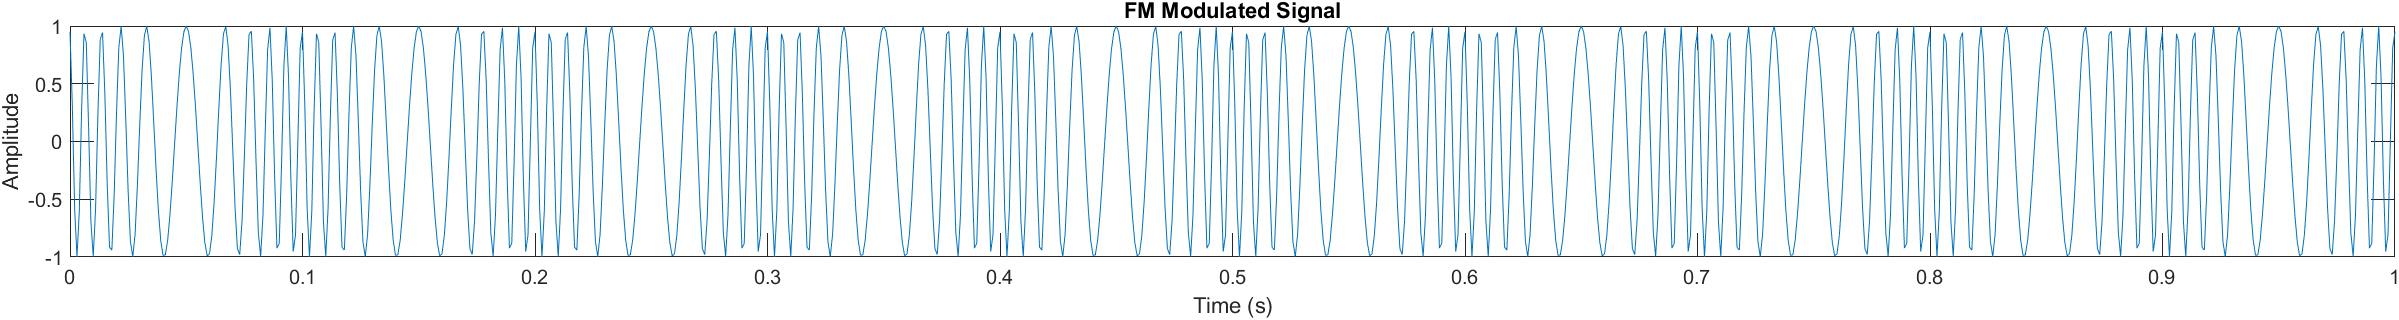
\includegraphics[width=\textwidth]{mod.png}
    \caption{FM Modulated Signal}
    \label{fig:img3}
\end{figure}

\begin{figure}[H]
    \centering
    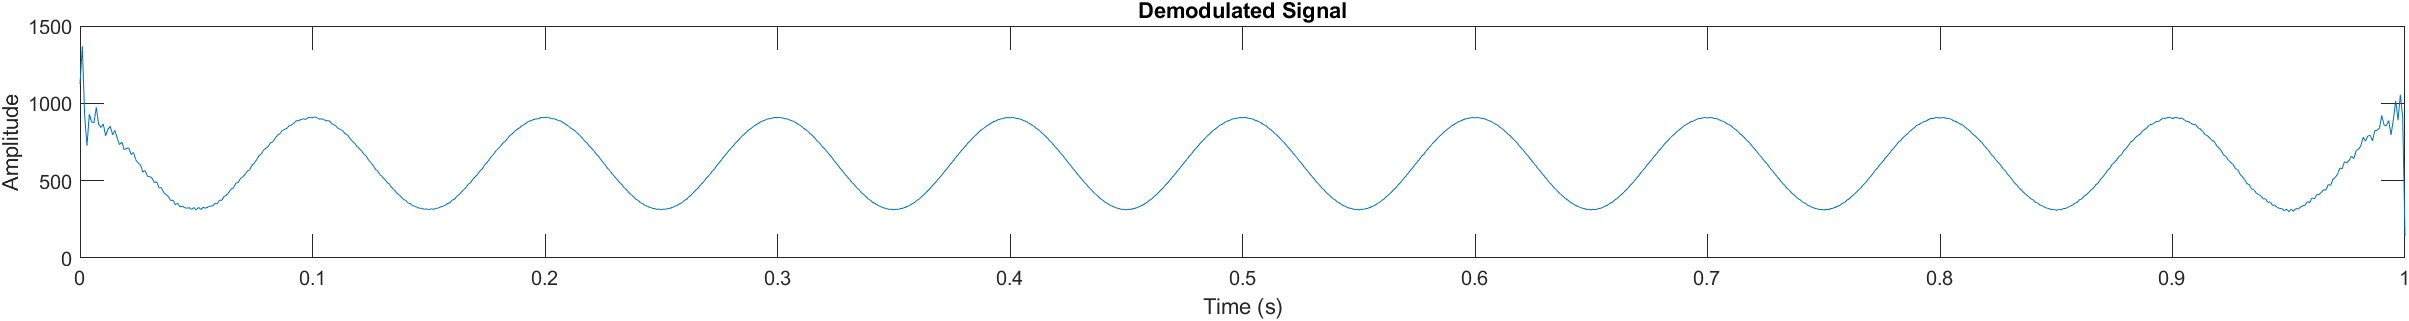
\includegraphics[width=\textwidth]{demod.png}
    \caption{Demodulated Signal}
    \label{fig:img4}
\end{figure}


\section*{Discussion}
\addcontentsline{toc}{section}{Discussion}
In this experiment, we explored the principles of Amplitude Modulation (AM) and Double Sideband Suppressed Carrier (DSB-SC) modulation and demodulation. The experimental data and Matlab simulations provided valuable insights into the behavior of these modulation techniques under different conditions.
\\\\
From the experimental data, we observed the following:
- For AM under modulation, the modulation index was calculated to be approximately 0.668. This indicates that the message signal's amplitude was less than the carrier amplitude, resulting in a modulated signal that did not fully utilize the carrier's amplitude range.
- For AM 100\% modulation, the modulation index was 1, indicating that the message signal's amplitude was equal to the carrier amplitude. This resulted in a modulated signal that fully utilized the carrier's amplitude range without distortion.
- For AM over modulation, the modulation index was calculated to be approximately 2.67. This indicates that the message signal's amplitude exceeded the carrier amplitude, resulting in a modulated signal with significant distortion, as observed in the waveforms.
\\\\
The Matlab simulations corroborated these findings by providing visual representations of the carrier, message, modulated, and demodulated signals for each modulation type. The simulations demonstrated the effects of under, 100\%, and over modulation on the AM signal and the successful demodulation of the original message signal.
\\\\
For DSB-SC modulation, the experimental data showed that the carrier was suppressed, and only the sidebands were transmitted. The Matlab simulations provided a clear visualization of the DSB-SC modulated signal and its demodulation process. The demodulated signals closely matched the original message signals, confirming the effectiveness of coherent detection in recovering the message from the DSB-SC modulated signal.
\\\\
Overall, this experiment highlighted the importance of the modulation index in AM and the efficiency of DSB-SC modulation in terms of power and bandwidth. The practical observations and simulations reinforced the theoretical concepts and provided a deeper understanding of these modulation techniques.

\section*{Conclusion}
\addcontentsline{toc}{section}{Conclusion}
In conclusion, this experiment provided a comprehensive understanding of Amplitude Modulation (AM) and Double Sideband Suppressed Carrier (DSB-SC) modulation techniques. Through both experimental observations and Matlab simulations, we were able to analyze the effects of different modulation indices on AM signals and the efficiency of DSB-SC modulation in terms of power and bandwidth. The results demonstrated the importance of the modulation index in determining the quality of AM signals and highlighted the advantages of DSB-SC modulation for efficient communication. These findings are consistent with the theoretical concepts discussed in the literature \cite{haykin2008communication, proakis2007digital}. Overall, this experiment reinforced the practical applications and benefits of these modulation techniques in communication systems.

\bibliographystyle{IEEEtran}
\renewcommand{\bibname}{References}
\addcontentsline{toc}{section}{References}
\bibliography{ref}

\end{document}
